\section{Shared-Bottom Baseline and Negative Transfer}
\subsection{Shared-Bottom Models}
The baseline model used in this review is the shared-bottom multi-task model. Its underlying principle can be traced back to Rich Caruana \citep{Caruana1997Multitask}, who argued that related tasks can benefit from one another through joint learning of shared representations that capture domain-specific information from the training signals. In modern deep multi-task recommendation, this principle is commonly instantiated through the shared-bottom architecture. As shown in Figure~\ref{fig:architectures}(a), this architecture contains several hidden layers following the input layer that are shared across all tasks. A task-specific tower is then built on top of the resulting shared representation for each task \citep{Ma2018MMoE}. 

Given $K$ tasks, the output of task $k$ can be formulated as
\begin{equation}
    y_k = h^k(f(x)),
    \label{eq:shared-bottom}
\end{equation}
where $f(\cdot)$ denotes the shared-bottom network and
$h^k(\cdot)$ denotes the task-specific tower for task $k$.

\begin{figure}[htbp]
\centering
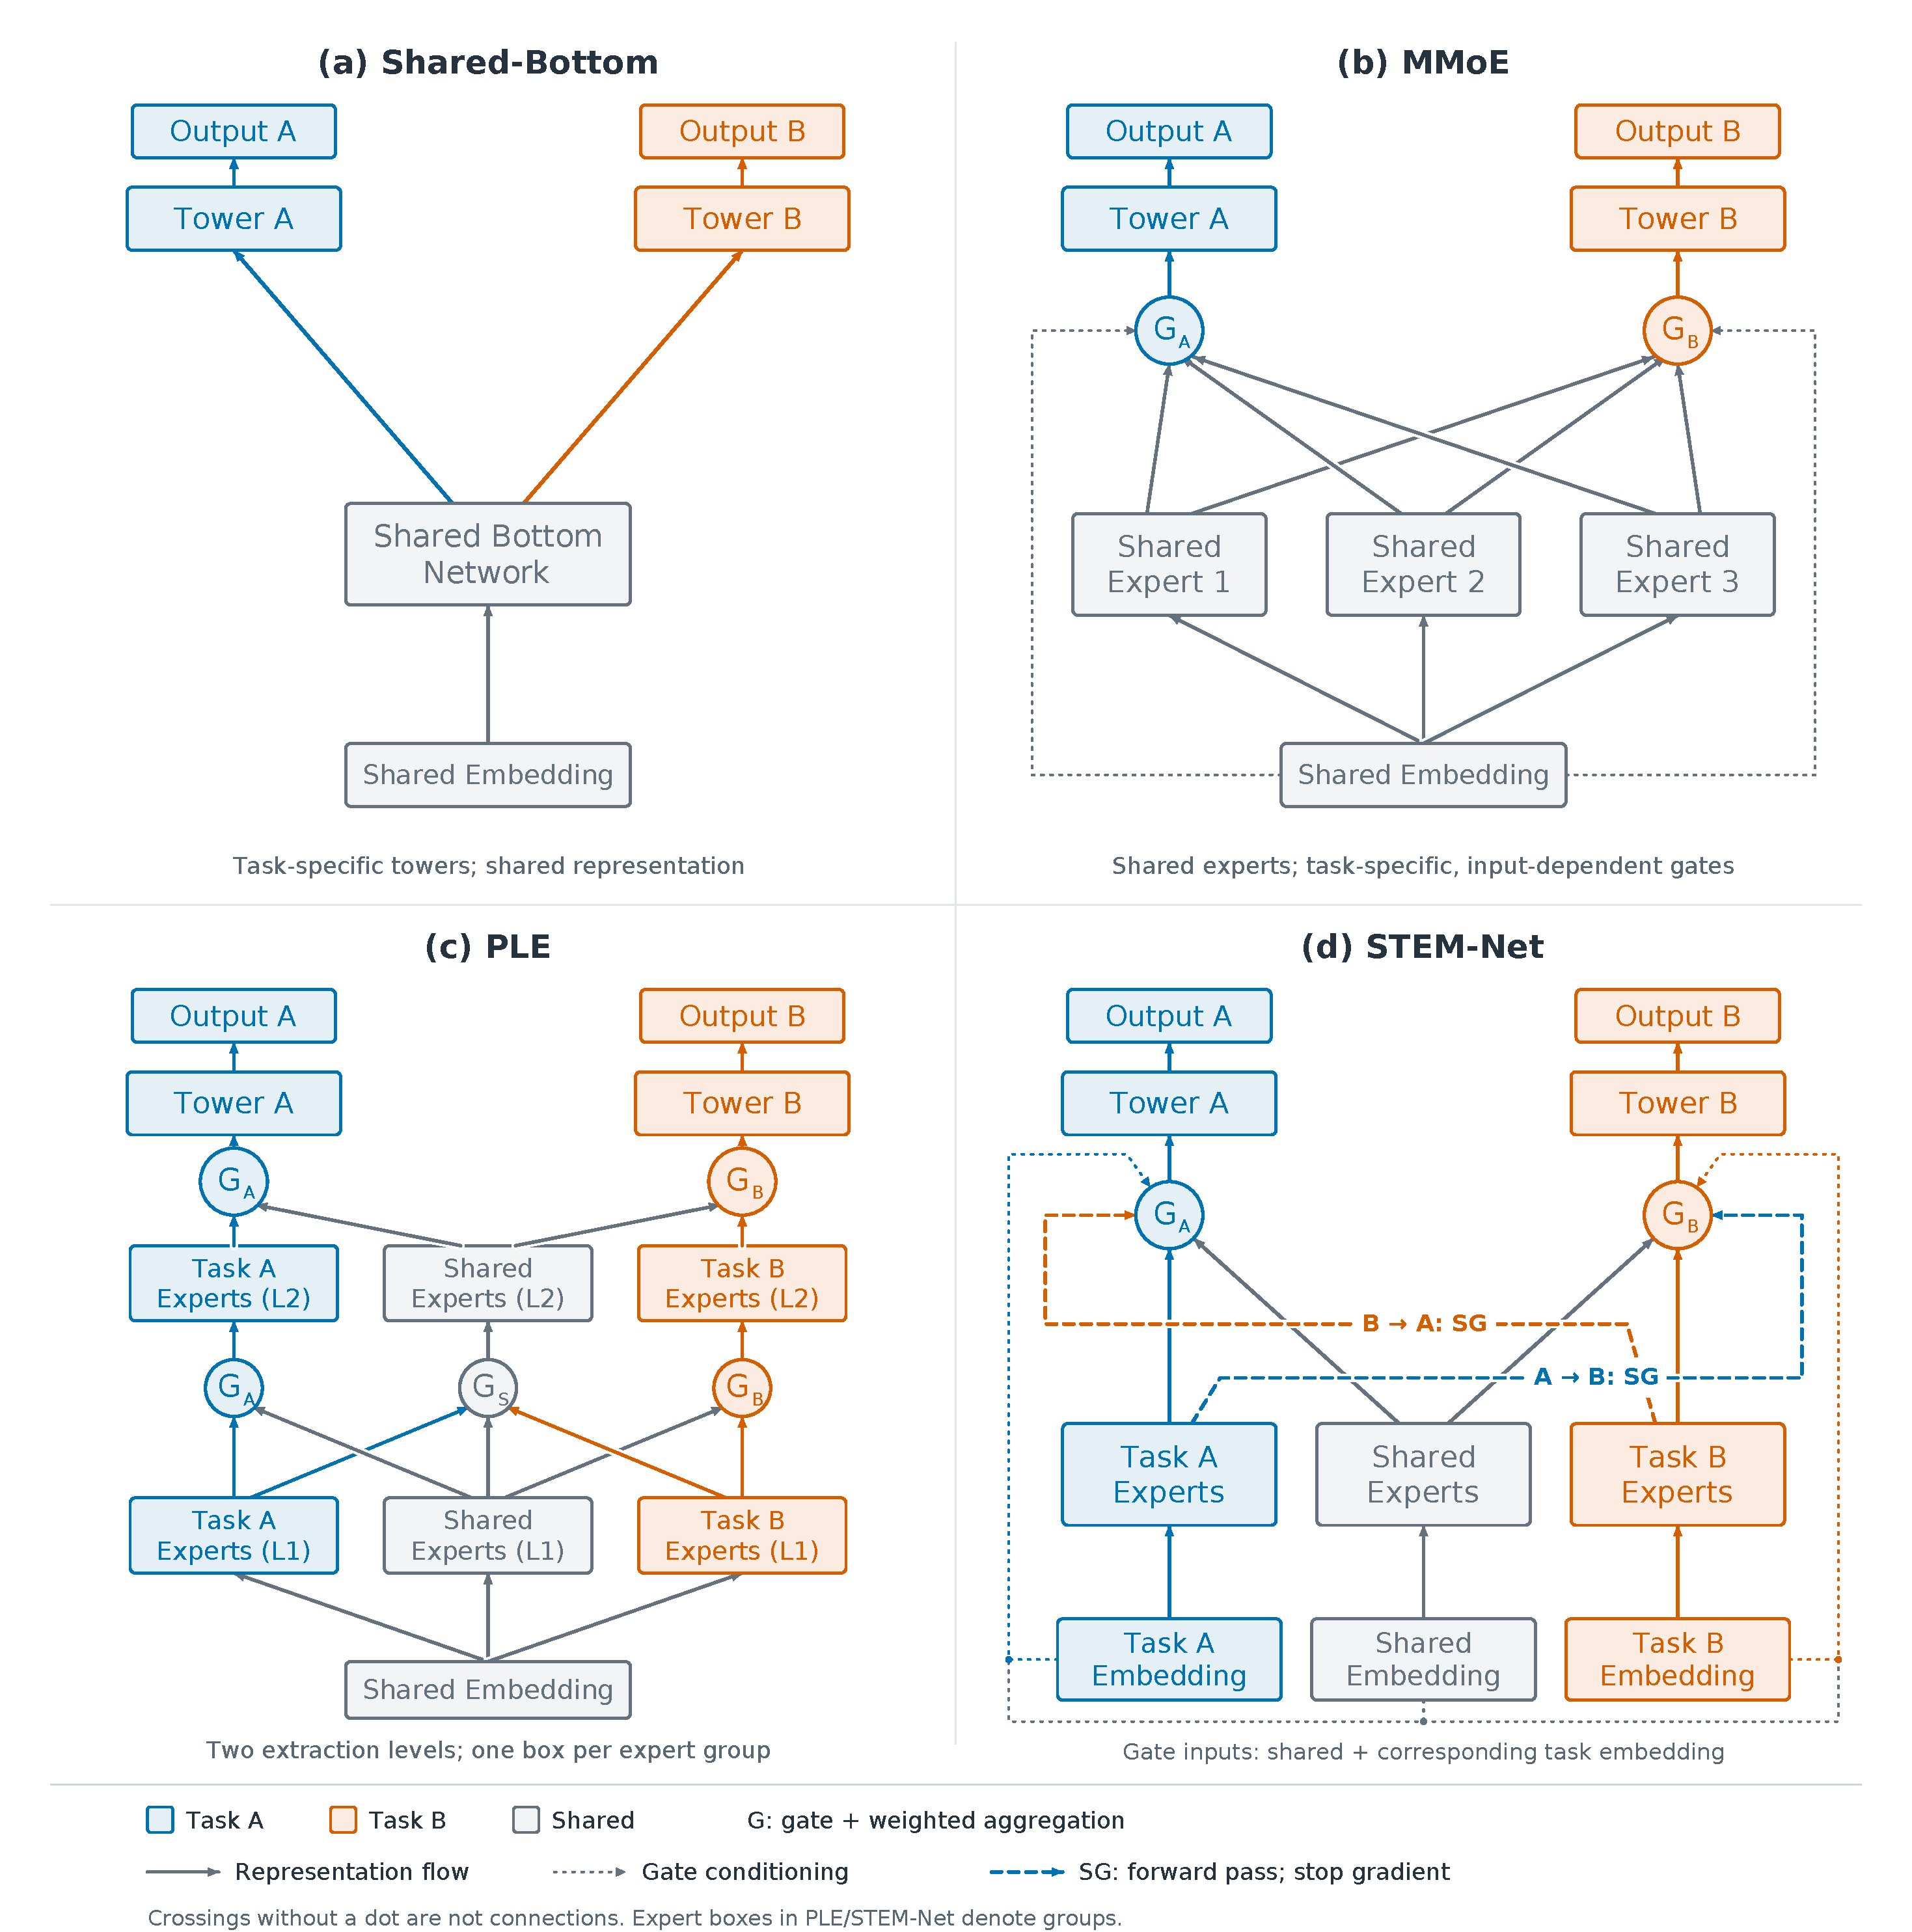
\includegraphics[height=0.62\textheight,keepaspectratio]{mtl_architectures.pdf}
\caption{Selective sharing architectures. Task-specific capacity moves from towers (a) to gates (b), experts (c), and embeddings (d). Line crossings without a junction dot do not indicate connections.}
\label{fig:architectures}
\end{figure}

\subsection{Negative Transfer}
\citet{BenDavid2008TaskRelatedness} theoretically formalised task relatedness as a key condition for the potential benefits of multitask learning (MTL). When task objectives are only partially aligned, sharing across tasks without accounting for their relatedness may lead to performance degradation, a phenomenon known as negative transfer \citep{pmlr-v48-leeb16, Wang2019NegativeTransfer}. Negative transfer in MTL can be explained through two important mechanisms. The first mechanism arises from gradient conflict, where different tasks generate conflicting or even opposing gradient directions when updating shared parameters, characterised by negative cosine similarity \citep{Yu2020PCGrad}. Another mechanism arises from gradient magnitude imbalance, where some tasks may generate substantially larger backpropagated gradients than others. This imbalance can cause certain tasks to dominate the updates of shared parameters, consequently distorting the joint optimisation process \citep{Chen2018GradNorm}. In the shared-bottom architecture, since all tasks share the same shared-bottom parameters under a fixed sharing structure regardless of task relatedness, the model may suffer from optimisation conflicts caused by task differences \citep{Ma2018MMoE}. 





